%Texlive-full Version 3.141592-1.40.3 (Web2C 7.5.6)
%Kile Version 2.0.83
%File associated : SoFa_Logo.ps , FF.ps

\documentclass[a4paper,10pt]{article}
\usepackage[utf8x]{inputenc}

\usepackage{lmodern}
\usepackage[a4paper]{geometry}
%\usepackage[frenchb]{babel}
\usepackage{graphicx}
\usepackage{hyperref}

\usepackage{pstricks}
\usepackage{pst-node}
%\usepackage{wrapfig}
\usepackage{amsmath}
\usepackage{amsfonts}
\usepackage{amssymb}
\usepackage{textcomp}

\usepackage{listings}
\lstset{language=C++,basicstyle=\scriptsize \color{green},identifierstyle=\color{orange},keywordstyle=[1]\color{blue},columns=fullflexible}

\usepackage{color}



\begin{document}
%%%%%%%%%%%%%%%%%%   LOGO  %%%%%%%%%%%%%%%%%%%%%%%%%
\begin{center}
\rput(6,1.5){\href{http://www.sofa-framework.org/}{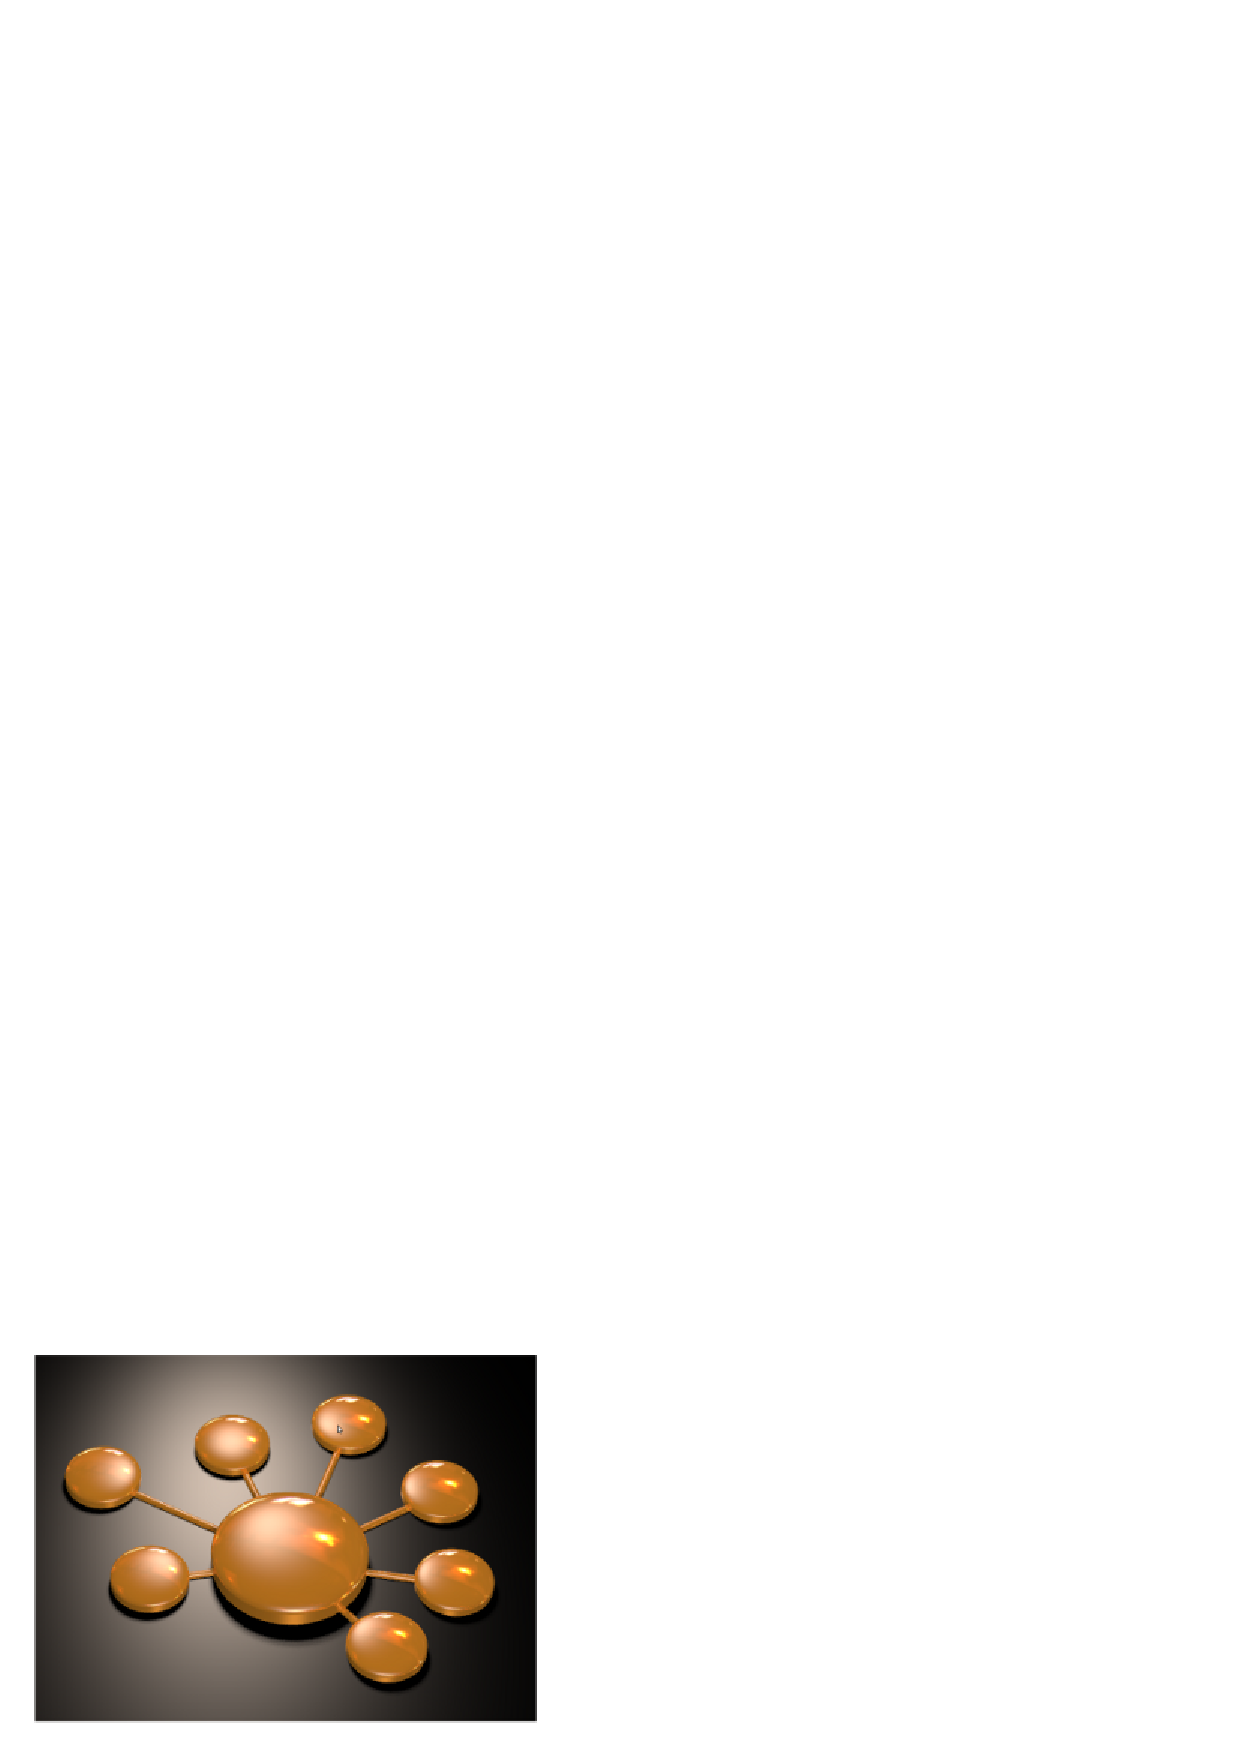
\includegraphics[scale=0.3]{SoFa_Logo}}}
\rput(-4,1.5){\href{http://www.sofa-framework.org/}{
		\begin{tabular}{l}
		\resizebox{4cm}{0.6cm}{SOFA} \\ 
		\resizebox{6cm}{0.3cm}{Simulation Open Framework Architecture}
		\end{tabular}
		}
	    }
\end{center}
%%%%%%%%%%%%%%%%%%   LOGO  %%%%%%%%%%%%%%%%%%%%%%%%%

%%%%%%%%%%%%%%%%%% DOCUMENT TITLE %%%%%%%%%%%%%%%%%%%%%%%%% To be deleted when include in the global document
%\chapter{Mapping} %\section{Rigid Mapping} 
\vspace{1.5cm}
\begin{center}\resizebox{7cm}{0.6cm}{FEM For Engeenering Material}\end{center}
%%%%%%%%%%%%%%%%%% DOCUMENT TITLE %%%%%%%%%%%%%%%%%%%%%%%%%

%%%%%%%%%%%%%%%%%%%%%%%%%%%%%%%%%%%%%%%%%%%%%%%%%%%%%%%%%%%%%%%%%%%%%%%%%%%%%%%%%%%%%%%%%
%=======================================================================================%
%%%%%%%%%%%%%%%%%%%%%%%%%%%%%%%%%%%%%%%%%%%%%%%%%%%%%%%%%%%%%%%%%%%%%%%%%%%%%%%%%%%%%%%%%
%\section{F.E.M}%%%%%%%%%%%%%%%%%%%%%%%

\section{FEM For Engeenering Material}

\paragraph{Abstract : }

\subsection{Equations for elastostatic: } 

\paragraph{Governing equations and Boundary problem: }
\paragraph{Variational formulation: }

\subsection{Equations for elastodynamic: }

\paragraph{Governing equations and Boundary problem: }
\paragraph{Variational formulation: }

\subsection{Interpolation: } 
Given a variational formulation in the integration formula :
\[
 \int_{\Omega} \left[\text{Integration Formula} \right]
\]
This integration can pass by the local integration :
\[
 \int_{\Omega} \left[\text{Integration Formula} \right] =\sum_{K} \int_{K} \left[\text{Integration Formula} \right] 
\]
Where $K$ is an Element. Now, interpolation allow to numerically compute this integration. To do this, we must to define several concept of Finite Element and also several convention of structure information. 
\paragraph{Conventions : } A Finite Element is a set of functions defined on a geometry elelemt which composed :
\begin{itemize}
\item A set of NbofDOF shape functions , usually polynomials.
\item A set of Node to be defined, usually NbofDOF=NbofNode. 
\end{itemize} 
In the rigorous, the number of shape funtions is equal to the number of degree of freedom. But in pratic, many shape function are alike. For exemple on tetrahedron, Finite Element linear : we have 4 nodes, in the dimension R3, so totally 12 degree of freedom. But for these 4 node, there are 4 polynomial to be defined, the rest is alike. That's why we must define some convention for the data structure. \\
For a displacement or a velocity field, there a two ways to presente by interpolation :
\begin{itemize}
\item Presentation by vector field : 
               \[\textbf{u}=\sum_{i=0}^{nbNode-1} \textbf{u}_i * {\bf\phi}_i  \]
\item Presentation by vector field : 
               \[\textbf{u}=\sum_{i=0}^{nbofDOF-1} u_i * \phi_i  \]
\end{itemize} 
In general, on the dimension RdDIM, we have nbofDOF=nbNode x RdDIM. A velocity or distribution field has nbofDOF scalar, which can be presented in two ways : an array of one dimention or two dimension. In the case array one dimensions, there are two presentation, depending to the order of each placed scalar. In the case array two demensions, there are also two presentation :   [nbNode x RdDIM] or [RdDIM x nbNode]. This brief view just make seen the diversity of structure, that must make a unique convention for a computation process. 
\paragraph{Conventions for scalar presentation : }
In the case RdDIM where there are nbofNode nodes, a vectorial field has nbofDOF = nbNode x RdDIM  value. The presentation of these values is :
               \[ \textbf{u}= u_0^0 u_1^0 u_2^0 ...  \]
\subsection{Integration: }

\subsection{Auto-test : }
These function on FEM are mostly linear transformation which is invertible. So we can verify all the computation, or pre-computation by the its inverted transformation. 
%%%%%%%%%%%%%%%%%%%%%%%%%%%%%%%%%%%%%%%%%%%%%%%%%%%%%%%%%%%%%%%%%%%%%%%%%%%%%%%%%%%%%  

						      %%%%%%%%%%%%%%%%%%%%%%%%%%  Writer %%%%%%%%%%%%%%%%%%%%%%%%
						      \begin{flushright}
						      Document written by \\
						      \href{mailto:chi-thanh.nguyen@inria.fr}{{\textbf {Chi Thanh NGUYEN}}} \\
						      INRIA Lille
						      \end{flushright}
						      %%%%%%%%%%%%%%%%%%%%%%%%%%  Writer %%%%%%%%%%%%%%%%%%%%%%%%

\end{document}
